\newpage
\exercice

Soient 4 points du plan $A$, $B$, $C$ et $D$.\\ $I$, $J$, $K$ et $L$ sont les milieux respectifs des côtés $[AB]$, $[BC]$, $[CD]$ et $[DA]$ du quadrilatère $ABCD$.\\

\begin{description}
	\item[Partie A :] conjecture\\
		Ouvrez un logiciel de géométrie dynamique.
		\begin{enumerate}
			\item Faites une figure.
			\item Déplacez les points $A$, $B$, $C$ ou $D$.\\ Que peut-on conjecturer~?
		\end{enumerate}
		Pour démontrer cette conjecture dans les parties suivantes, on choisit de définir un repère et d'exprimer les coordonnées des points dans ce repère.\\
		
	\item[Partie B :] un cas particulier\\
		Soit le repère\rep{A}{B}{D}. Dans cette partie, les points sont disposés comme sur la figure ci-dessous, aux n\oe{}uds du réseau.
		\begin{center}
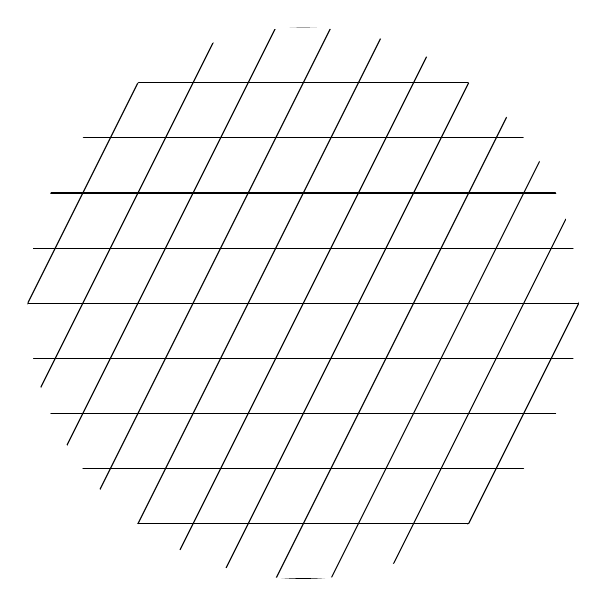
\begin{tikzpicture}[scale=0.7,every node/.style={scale=0.7}]
\placerpoint{A}{0}{0}{above left};
\placerpoint{B}{4}{0}{below right};
\placerpoint{C}{7.5}{5}{below right};
\placerpoint{D}{1}{2}{above left};
%\clip (-2,-0.1) rectangle (9,5.5);
\clip (4,2) circle (5);
%\foreach \y in {0, 1, ..., 10}{
	\foreach \x in {-10, ..., 10}{
		\begin{scope}[xshift=\x cm]
			\draw (-10,-20) -- (10,20);
		\end{scope}
		\begin{scope}[yshift=\x cm]
			\draw (-20,0) -- (20,0);
		\end{scope}
	}
%}
\end{tikzpicture}
\end{center}
		\begin{enumerate}
			\item Donnez les coordonnées des points $A$, $B$, $C$ et $D$.
			\item Calculez les coordonnées des milieux $I$, $J$, $K$ et $L$.
			\item Démontrez la conjecture de la partie précédente dans ce cas particulier.\\
		\end{enumerate}
		
	\item[Partie C :] cas général\\
		Soit le repère\rep{A}{B}{D} et on note$\pointcoord{~}{a}{b}$ les coordonnées du point $C$ dans ce repère.
		\begin{enumerate}
			\item Calculez les coordonnées des milieux $I$, $J$, $K$ et $L$ en fonction de $a$ et $b$.
			\item Démontrez la conjecture.\\
		\end{enumerate}
		
	\item[Partie D :] sans coordonnées\\
		Comment aurait-on pu démontrer ce théorème sans utiliser les coordonnées~?\\
\end{description}